%%%%%%%%%%%%%%%%%%%%%%%%%%%%%%%%%%%%%%%%%
% Thin Sectioned Essay
% LaTeX Template
% Version 1.0 (3/8/13)
%
% This template has been downloaded from:
% http://www.LaTeXTemplates.com
%
% Original Author:
% Nicolas Diaz (nsdiaz@uc.cl) with extensive modifications by:
% Vel (vel@latextemplates.com)
%
% License:
% CC BY-NC-SA 3.0 (http://creativecommons.org/licenses/by-nc-sa/3.0/)
%
%%%%%%%%%%%%%%%%%%%%%%%%%%%%%%%%%%%%%%%%%

%----------------------------------------------------------------------------------------
%	PACKAGES AND OTHER DOCUMENT CONFIGURATIONS
%----------------------------------------------------------------------------------------

\documentclass[a4paper, 12pt]{article} % Font size (can be 10pt, 11pt or 12pt) and paper size (remove a4paper for US letter paper)
\usepackage[portuguese]{babel}

\usepackage[protrusion=true,expansion=true]{microtype} % Better typography
\usepackage{graphicx} % Required for including pictures
\usepackage{wrapfig} % Allows in-line images

\usepackage{mathpazo} % Use the Palatino font
\usepackage[T1]{fontenc} % Required for accented characters
\linespread{1.05} % Change line spacing here, Palatino benefits from a slight increase by default
\usepackage{float}
\makeatletter
\renewcommand\@biblabel[1]{\textbf{#1.}} % Change the square brackets for each bibliography item from '[1]' to '1.'
\renewcommand{\@listI}{\itemsep=0pt} % Reduce the space between items in the itemize and enumerate environments and the bibliography

\renewcommand{\maketitle}{
\begin{titlepage}
    \begin{center}
        \vspace*{1cm}
        
\includegraphics[width=0.35\textwidth]{../images/logo-no-bg.png}\\[1cm] % Logo
        {\Huge\textbf{Vizzy - Plataforma Comunitária}}\\[0.5cm] % Main Title
        {\Large Projeto de Desenvolvimento de Software}\\[2cm] % Subtitle
        {\large \textsc{
        Enrique Rodrigues Nº28602 \\
        José Alves Nº27967 \\
        Diogo Machado Nº26042 \\
        Diogo Abreu Nº27975 \\
        André Silva Nº27965}}\\[0.5cm] % Authors
        {\textit{Instituto Politécnico do Cávado e do Ave}}\\[1.5cm] % Institution
        {\large \today} % Date
        \vfill
        % \textbf{Keywords:} lorem, ipsum, dolor, sit amet, lectus % Keywords
    \end{center}
\end{titlepage}
}
\makeatother

%----------------------------------------------------------------------------------------
%	TITLE
%----------------------------------------------------------------------------------------

\title{\textbf{Vizzy - Plataforma Comunitária}\\ % Title
	Projeto de Desenvolvimento de Software} % Subtitle

\author{
	\textsc{Enrique Rodrigues Nº28602}, \\
	\textsc{José Alves}, \\
	\textsc{Diogo Machado}, \\
	\textsc{Diogo Abreu Nº27975}, \\ 
	\textsc{André Silva} \\
	\textit{Instituto Politécnico do Cávado e do Ave}
}

\date{\today} % Date

%------------------------------------------------------------------------------------

\begin{document}

\maketitle % Print the title section

%----------------------------------------------------------------------------------------
%	ABSTRACT AND KEYWORDS
%----------------------------------------------------------------------------------------

%\renewcommand{\abstractname}{Summary} % Uncomment to change the name of the abstract to something else

% \begin{abstract}
% Morbi tempor congue porta. Proin semper, leo vitae faucibus dictum, metus mauris lacinia lorem, ac congue leo felis eu turpis. Sed nec nunc pellentesque, gravida eros at, porttitor ipsum. Praesent consequat urna a lacus lobortis ultrices eget ac metus. In tempus hendrerit rhoncus. Mauris dignissim turpis id sollicitudin lacinia. Praesent libero tellus, fringilla nec ullamcorper at, ultrices id nulla. Phasellus placerat a tellus a malesuada.
% \end{abstract}

% \hspace*{3,6mm}\textit{Keywords:} lorem , ipsum , dolor , sit amet , lectus % Keywords

% \vspace{30pt} % Some vertical space between the abstract and first section

%----------------------------------------------------------------------------------------
%	DOCUMENT BODY
%----------------------------------------------------------------------------------------

\newpage
\section{Introdução}

A Vizzy é uma plataforma comunitária desenvolvida para facilitar a compra, venda, troca e aluguer de itens entre pessoas da mesma comunidade, promovendo uma forma prática, económica e sustentável de partilhar recursos.

Através da Vizzy, os utilizadores podem adquirir produtos em segunda mão, trocar itens ou até alugar ferramentas e outras coisas. Isto não só reduz o desperdício, mas também oferece uma alternativa mais acessível, especialmente quando se trata de alugueres. Alugar uma ferramenta a um vizinho, por exemplo, pode ser muito mais económico do que comprá-la a uma grande empresa.

O objetivo da plataforma é criar uma rede de partilha dentro da comunidade, onde os membros possam beneficiar de um consumo mais consciente, poupando dinheiro e recursos, ao mesmo tempo que promovem a sustentabilidade e a cooperação.

Neste relatório, serão apresentados os principais detalhes da aplicação, incluindo diagramas UML e mockups, que ilustram as funcionalidades essenciais da Vizzy.

\newpage
\section{Problema e Motivação}

\subsection{O Problema}

Nos dias de hoje, muitas comunidades enfrentam desafios económicos e ambientais relacionados ao consumo excessivo e à falta de acesso a certos produtos. Itens valiosos acabam por ser desperdiçados ou ficam esquecidos, enquanto outras pessoas na mesma comunidade poderiam beneficiar deles. Ao mesmo tempo, a aquisição de novos produtos nem sempre é uma opção viável devido ao custo ou à disponibilidade limitada.

Outro desafio importante é a falta de soluções práticas para facilitar a troca, venda e aluguer de itens de forma organizada, o que leva a um ciclo de consumo ineficiente e desperdício de recursos.

\subsection{A Solução Proposta}

A Vizzy surge como uma resposta a estes problemas, oferecendo uma plataforma onde os membros da comunidade podem comprar, vender, trocar e alugar itens de forma simples e segura. Com esta solução, é possível dar uma segunda vida a produtos que seriam descartados e permitir que as pessoas acedam a bens de que necessitam, sem precisarem de comprá-los novos.

Além disso, ao permitir o aluguer de ferramentas e outros objectos, a Vizzy oferece uma alternativa económica e prática, como no caso de alugar uma ferramenta a um vizinho em vez de recorrer a grandes empresas. Isto não só reduz os custos para os utilizadores, mas também contribui para um modelo de consumo mais sustentável.

A plataforma visa, assim, otimizar o uso dos recursos, reduzir desperdícios e fortalecer os laços entre os membros da comunidade. Com a Vizzy, todos podem beneficiar de uma forma mais acessível e consciente de consumir, promovendo a circularidade e a sustentabilidade.

%------------------------------------------------------------------------------------

\newpage
\section{Processos de Negócio}

\subsection{Processo de Empréstimo/Aluguer}

\subsubsection{Etapas}
\begin{itemize}
	\item \textbf{Criar um produto}: O utilizador adiciona um produto à plataforma, fornecendo detalhes como nome, descrição, estado e fotos.
	\item \textbf{Definir datas bloqueadas}: O utilizador indica as datas em que o produto não estará disponível para empréstimo/aluguer.
	\item \textbf{Confirmar datas livres}: O sistema verifica e confirma as datas disponíveis para empréstimo/aluguer com base nas datas bloqueadas.
	\item \textbf{Definir valor associado}: O utilizador define o valor do aluguer (ou 0€ em caso de empréstimo).
	\item \textbf{O produto não desaparece}: Após o empréstimo/aluguer, o produto permanece na plataforma para futuras transações.
\end{itemize}

\subsubsection{Fluxo de Trabalho}
O utilizador cria o produto e define as datas disponíveis. Outros utilizadores podem solicitar o empréstimo/aluguer nas datas livres. O proprietário do produto confirma ou rejeita a solicitação. Após o uso, o produto volta a estar disponível na plataforma.

\subsubsection{Interações Essenciais}
\begin{itemize}
	\item Possibilidade de elogiar o vendedor após o empréstimo/aluguer para garantir a qualidade do serviço.
\end{itemize}

\section{Processo de Venda}

\subsubsection{Etapas}
\begin{itemize}
	\item \textbf{Criar um produto}: O utilizador adiciona um produto à plataforma com detalhes como nome, descrição, estado e fotos.
	\item \textbf{Definir um valor associado}: O utilizador define o preço de venda do produto.
	\item \textbf{Permitir ou não receber contrapropostas}: O utilizador decide se aceita ou não contrapropostas de outros utilizadores.
	\item \textbf{Aceitar/Rejeitar contrapropostas}: Se permitido, o vendedor pode aceitar ou rejeitar contrapropostas recebidas.
	\item \textbf{Concretizada a venda, o produto desaparece}: Após a venda, o produto é marcado como vendido.
\end{itemize}

\subsubsection{Fluxo de Trabalho}
O utilizador cria o produto e define o preço. Outros utilizadores podem comprar diretamente ou fazer contrapropostas (se permitido). O vendedor aceita ou rejeita as propostas. Após a venda, o produto é removido da plataforma.

\subsection{Processo de Troca}

\subsubsection{Etapas}
\begin{itemize}
	\item \textbf{Criar um produto}: O utilizador adiciona um produto à plataforma com detalhes como nome, descrição, estado e fotos.
	\item \textbf{Associar um produto para troca}: O utilizador indica qual produto deseja receber em troca.
	\item \textbf{Fazer contrapropostas}: Outros utilizadores podem fazer contrapropostas com produtos diferentes.
	\item \textbf{Aceitar/Rejeitar contrapropostas}: O utilizador pode aceitar ou rejeitar as contrapropostas recebidas.
\end{itemize}

\subsubsection{Fluxo de Trabalho}
O utilizador cria o produto e indica o produto desejado em troca.O utilizador aceita ou rejeita as propostas. Após a troca, ambos os produtos são removidos da plataforma.

\subsection{Integração dos Processos}

\subsubsection{Interações entre Processos}
\begin{itemize}
	\item \textbf{Empréstimo/Aluguer e Venda}: Um produto pode estar disponível para empréstimo ou venda,após a venda ele é marcado como vendido.
	\item \textbf{Troca e Venda}: Um produto pode ser oferecido para troca ou venda, mas o utilizador deve escolher uma das opções.
	\item \textbf{Avaliações}: Todos os usuários vão ter a possibilidade de colocar um "elogio" no vendedor após-transação para garantir a qualidade e confiança na plataforma. 
\end{itemize}

\subsubsection{Fluxo Geral}
\begin{itemize}
	\item O utilizador escolhe o tipo de transação (empréstimo/aluguer, venda ou troca).
	\item O utilizador cria o produto e define os detalhes específicos para cada processo.
	\item Outros utilizadores interagem com o produto (solicitam empréstimo, compram ou propõem trocas).
	\item O proprietário do produto confirma ou rejeita as solicitações.
	\item Após a transação, o produto é marcado como vendido ou permanece disponível (empréstimo/aluguer).
\end{itemize}

%------------------------------------------------------------------------------------

\newpage
\section{Requisitos Funcionais}
Os requisitos funcionais \textbf{(RFs)} são as especificações que definem o que um sistema deve fazer para atender às necessidades dos utilizadores. Eles descrevem as funcionalidades, comportamentos e operações que o sistema deve oferecer, incluindo interações entre utilizadores e o sistema, processamento de dados e regras de negócio.

\begin{table}[H]
	\centering
	\renewcommand{\arraystretch}{1.3}
	\begin{tabular}{|c|p{12cm}|}
		\hline
		\textbf{Código} & \textbf{Requisito Funcional} \\
		\hline
		\textbf{RF 01} & O utilizador pode criar um anúncio na aplicação, fornecendo nome, descrição, estado do produto, fotos e definir se é para venda, troca ou empréstimo/aluguer. \\
		\hline
		\textbf{RF 02} & O utilizador pode definir datas bloqueadas para empréstimo/aluguer do produto. \\
		\hline
		\textbf{RF 03} & O sistema deve verificar e confirmar as datas livres para empréstimo/aluguer. \\
		\hline
		\textbf{RF 04} & O utilizador pode definir um valor para aluguer ou venda. \\
		\hline
		\textbf{RF 05} & O utilizador pode permitir ou não propostas nos anúncios. \\
		\hline
		\textbf{RF 06} & O utilizador pode aceitar, rejeitar ou negociar propostas. \\
		\hline
		\textbf{RF 07} & Após a transação de um produto para venda ou troca, o anúncio deve ser marcado como concluído e deixar de aparecer para os outros utilizadores. \\
		\hline
		\textbf{RF 08} & O utilizador ao criar um anúncio para troca pode indicar qual produto deseja receber em troca. \\
		\hline
		\textbf{RF 09} & A aplicação deve permitir a pesquisa de produtos disponíveis na plataforma. \\
		\hline
		\textbf{RF 10} & O utilizador pode adicionar produtos a uma lista de favoritos. \\
		\hline
		\textbf{RF 11} & A aplicação deve garantir a segurança dos dados dos utilizadores e transações. \\
		\hline
	\end{tabular}
	\caption{Requisitos Funcionais}
	\label{tab:requisitos_funcionais}
\end{table}

%------------------------------------------------------------------------------------

\newpage
\section{Requisitos Não Funcionais}

Os requisitos não funcionais \textbf{(RNFs)} definem as características e restrições de um sistema que não estão diretamente relacionadas às funcionalidades oferecidas, mas sim à qualidade, desempenho, segurança e usabilidade da aplicação. Eles garantem que o sistema seja eficiente, confiável e utilizável dentro de determinados padrões.

\begin{table}[H]
	\centering
	\renewcommand{\arraystretch}{1.3}
	\begin{tabular}{|c|p{12cm}|}
		\hline
		\textbf{Código} & \textbf{Requisito Não Funcional} \\
		\hline
		\textbf{RNF 01} & A interface do utilizador deve ser intuitiva e acessível para todas as faixas etárias. \\
		\hline
		\textbf{RNF 02} & Todos os dados dos utilizadores devem ser armazenados de forma segura. \\
		\hline
		\textbf{RNF 03} & 	A aplicação deve cumprir com o Regulamento Geral de Proteção de Dados (RGPD) da União Europeia, garantindo a privacidade e o consentimento para o uso de dados pessoais. \\
		\hline
		\textbf{RNF 04} & O tempo de carregamento do feed da aplicação não deve ultrapassar os 3 segundos. \\
		\hline
		\textbf{RNF 05} & A pesquisa de produtos deve devolver os resultados em menos de 5 segundos.\\
		\hline
		\textbf{RNF 06} & O sistema deve permitir a implementação de novas funcionalidades com um impacto mínimo no desempenho. \\
		\hline
		\textbf{RNF 07} & A aplicação deve exigir uma palavra-passe com pelo menos 8 caracteres, incluindo letras e números. \\
		\hline
		\textbf{RNF 08} & O sistema deve utilizar armazenamento em cache para reduzir o número de pedidos ao servidor e melhorar a eficiência. \\
		\hline
		\textbf{RNF 09} & O sistema deve limitar o tamanho máximo de imagens carregadas para 5MB, evitando uso excessivo de espaço. \\
		\hline
	\end{tabular}
	\caption{Requisitos Não Funcionais}
	\label{tab:requisitos_nao_funcionais}
\end{table}

%------------------------------------------------------------------------------------

\newpage

\section{Arquitetura}
A arquitetura da plataforma é composta por um frontend desenvolvido com \textbf{React e Next.js}, um backend em \textbf{C\#}, e uma base de dados gerida com \textbf{Supabase (PostgreSQL)}. Esta abordagem garante um sistema eficiente, seguro e escalável.

\begin{figure}[ht]
	\centering
	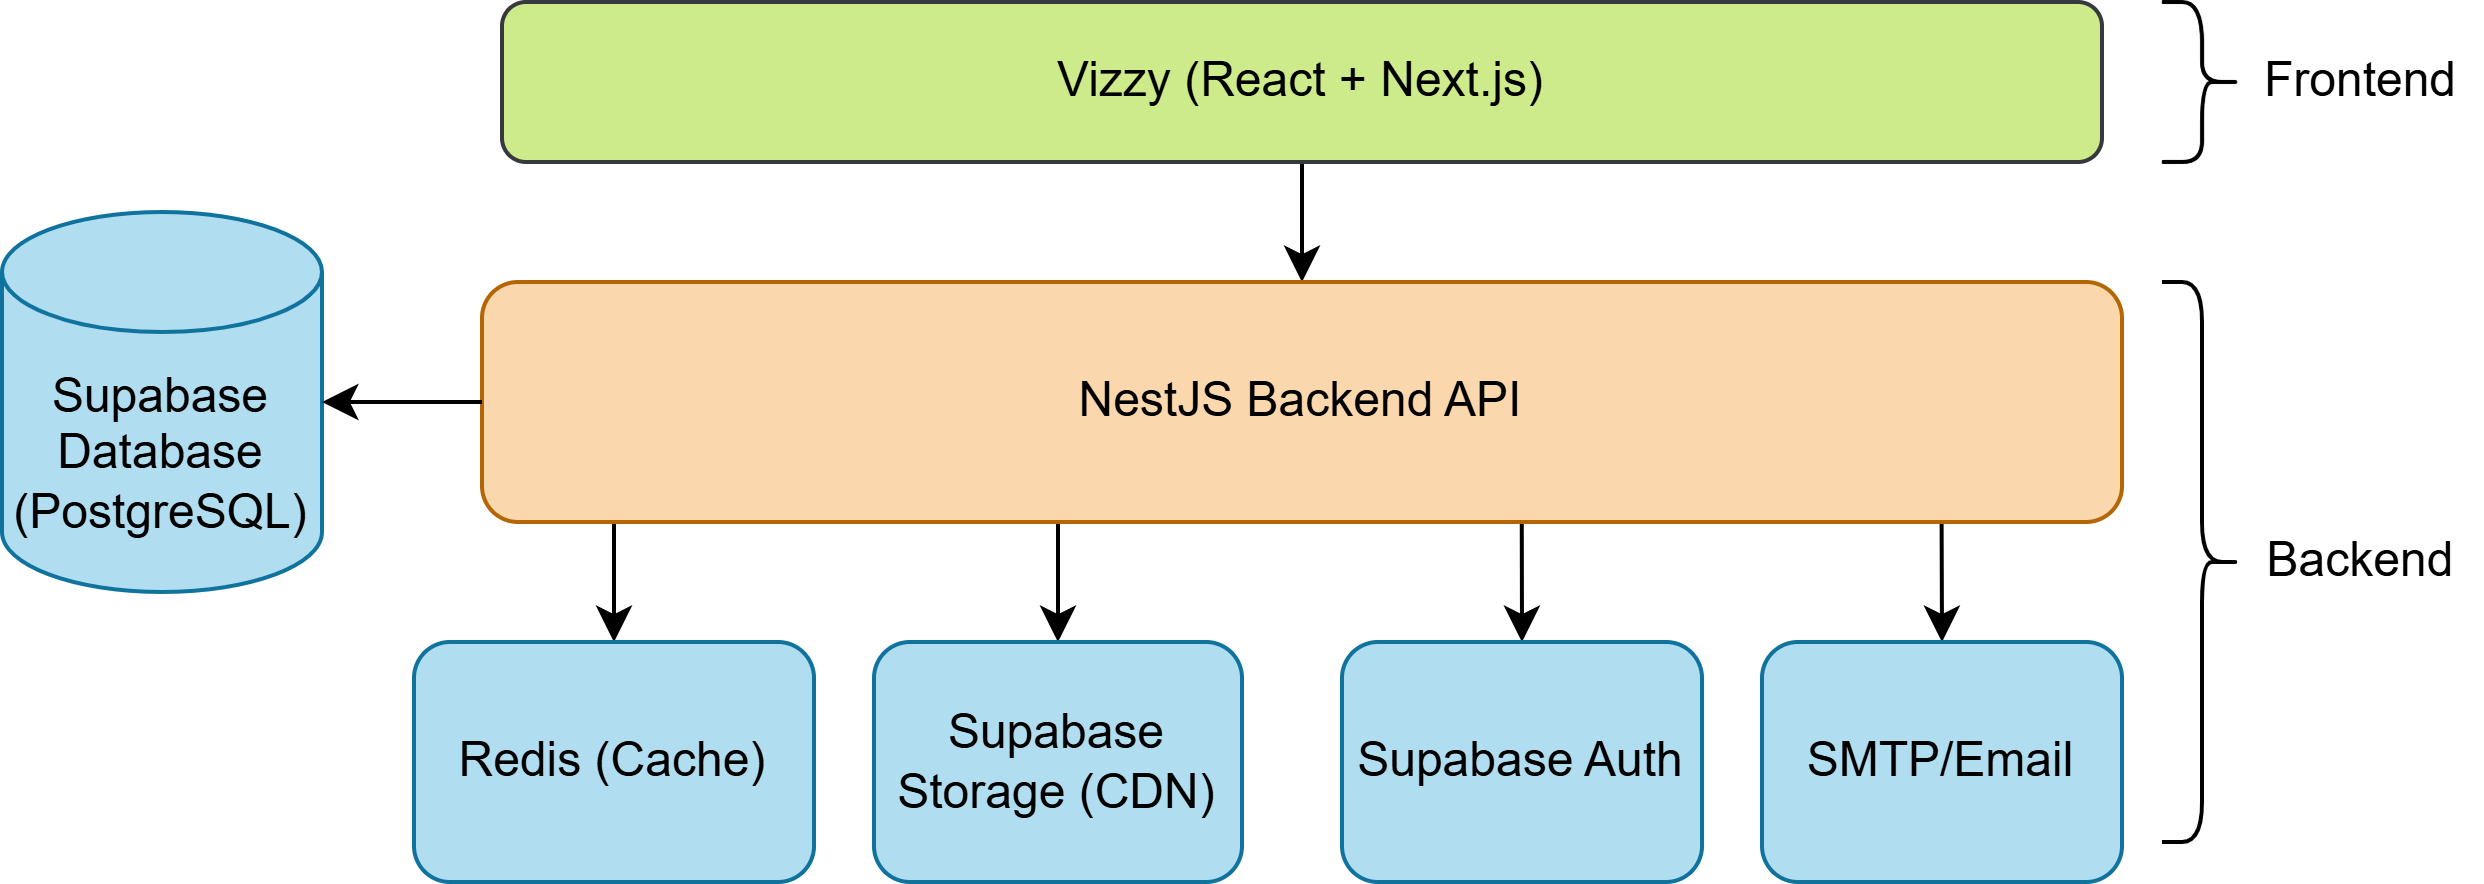
\includegraphics[width=\textwidth]{../images/system-architecture.png}
	\caption{Arquitetura da Plataforma}
	\label{fig:arquitetura}
\end{figure}

\subsection{Frontend}
O frontend foi desenvolvido com \textbf{Next.js} para tirar proveito do server-side rendering (SSR) e static site generation (SSG), o que melhora o desempenho e o SEO. Além disso, o sistema utiliza API Routes para comunicação eficiente com o backend e otimização de carregamento de páginas para melhor experiência do utilizador.

\subsection{Backend}
O backend é composto por diversos serviços que trabalham em conjunto para garantir a funcionalidade da plataforma:

\begin{itemize}
	\item \textbf{API Backend (C\#):} Responsável pelo processamento dos pedidos HTTP do frontend, gestão de dados e comunicação com a base de dados.
	\item \textbf{Supabase Auth:} Sistema de autenticação e gestão de utilizadores, garantindo segurança no acesso à plataforma.
	\item \textbf{SMTP/Email:} Serviço de envio de emails para notificações e recuperação de credenciais.
	\item \textbf{Supabase Storage (CDN):} Sistema de armazenamento utilizado para gerir ficheiros e recursos estáticos.
\end{itemize}

\subsection{Base de Dados}
A plataforma utiliza o \textbf{PostgreSQL} como base de dados relacional. Esta base de dados oferece alta escalabilidade, confiabilidade e desempenho, permitindo operações eficientes de leitura e escrita.

\subsection{Fluxo de Funcionamento}
\begin{enumerate}
	\item O utilizador interage com o \textbf{frontend (Vizzy)}.
	\item Os pedidos são enviados para o \textbf{API Backend (C\#)}, que os processa e consulta a base de dados.
	\item A autenticação é gerida pelo \textbf{Supabase Auth}, garantindo a segurança no acesso.
	\item Os ficheiros carregados são armazenados no \textbf{Supabase Storage (CDN)}.
	\item O serviço de email (SMTP) é utilizado principalmente para a recuperação de senhas e outras funcionalidades de gestão de contas, como confirmação de registo e redefinição de credenciais.
\end{enumerate}

Esta arquitetura assegura um sistema robusto, seguro e otimizado, permitindo uma gestão eficiente dos recursos e uma experiência fluida para os utilizadores.

%------------------------------------------------
\newpage
\section*{\textit{Product Backlog}}

A plataforma pr

%------------------------------------------------
\newpage
\section*{\textit{User Stories}}
\subsection{}
A plataforma pr

%------------------------------------------------
\newpage
\section*{Diagrama de caso de Uso}

A plataforma pr
%------------------------------------------------
\newpage
\section*{Diagrama BPMN}

A plataforma pr


%------------------------------------------------
\newpage
\section*{Diagrama ER}

O diagrama representa um software de produtos onde os utilizadores podem comprar, vender, alugar ou trocar. A estrutura do modelo de dados é composta por várias tabelas interligadas, refletindo diferentes tipos de listagens, propostas e transações.

\textbf{Principais Tabelas e Ligações}

\textbf{1. Utilizadores (User)}

\begin{itemize}
    \item Esta tabela armazena informações dos utilizadores, incluindo nome, email, data de criação e último acesso.
    \item Está ligada a várias tabelas, incluindo:
    \begin{itemize}
        \item \textbf{Location} (localização do utilizador)
        \item \textbf{UserType} (tipo de utilizador)
        \item \textbf{BlockedUser} (bloqueios entre utilizadores)
        \item \textbf{Favorite} (itens favoritos do utilizador)
        \item \textbf{Proposal} (propostas enviadas e recebidas)
        \item \textbf{UserTransaction} (transações associadas ao utilizador)
    \end{itemize}
\end{itemize}
\textbf{2. Listagens (Listing)}

\begin{itemize}
    \item Representa os itens que os utilizadores podem colocar na plataforma para venda, aluguer, troca ou venda.
    \item Campos principais incluem título, descrição, data de criação, estado do anúncio e categoria.
    \item Está ligada às seguintes tabelas:
    \begin{itemize}
        \item \textbf{ListingStatus} (estado da listagem)
        \item \textbf{Category} (categoria da listagem)
        \item \textbf{User} (dono da listagem)
        \item \textbf{Favorite} (itens marcados como favoritos pelos utilizadores)
        \item Tipos específicos de listagens: \textbf{SaleListing}, \textbf{RentalListing}, \textbf{SwapListing} e \textbf{GiveawayListing}.
    \end{itemize}
\end{itemize}
\textbf{3. Tipos de Listagens}

\begin{itemize}
    \item \textbf{SaleListing}: Inclui preço, condição do item e se é negociável.
    \item \textbf{RentalListing}: Contém informações sobre custo diário, data de indisponibilidade e taxa de atraso.
    \item \textbf{SwapListing}: Define a categoria e o item desejado para troca.
    \item \textbf{GiveawayListing}: Especifica requisitos para quem pode receber o item gratuitamente.
\end{itemize}
\textbf{4. Propostas (Proposal)}

\begin{itemize}
    \item Esta tabela armazena propostas de transação entre utilizadores, incluindo envio e receção.
    \item Está ligada a:
    \begin{itemize}
        \item \textbf{ProposalType} (tipo de proposta)
        \item \textbf{User} (remetente e destinatário)
        \item \textbf{Listing} (listagem associada)
        \item Tipos específicos de propostas: \textbf{SaleProposal}, \textbf{RentalProposal}, \textbf{SwapProposal} e \textbf{GiveawayProposal}.
    \end{itemize}
\end{itemize}
\textbf{5. Transações (Transaction)}

\begin{itemize}
    \item Regista as transações concretizadas na plataforma.
    \item Campos principais incluem data da transação, estado, utilizador envolvido e proposta associada.
    \item Está ligada a:
    \begin{itemize}
        \item \textbf{TransactionStatus} (estado da transação)
        \item \textbf{Listing} (item envolvido)
        \item \textbf{Proposal} (proposta que originou a transação)
        \item \textbf{UserTransaction} (relação entre comprador e vendedor).
    \end{itemize}
\end{itemize}
\textbf{6. Outras tabelas de suporte}

\begin{itemize}
    \item \textbf{Location} e \textbf{Contact}: Guardam detalhes sobre localização e contactos de empresas.
    \item \textbf{Category}: Define categorias para as listagens.
    \item \textbf{BlockedUser}: Armazena relações de bloqueio entre utilizadores.
    \item \textbf{UserType}: Define diferentes tipos de utilizadores (por exemplo, comprador, vendedor, administrador).
\end{itemize}

Este diagrama ER modela um sistema robusto para compra, venda, aluguer e troca de itens. As tabelas principais são \textbf{User}, \textbf{Listing}, \textbf{Proposal} e \textbf{Transaction}, com relações bem definidas para manter a integridade dos dados.


\begin{figure}[ht]
	\centering
	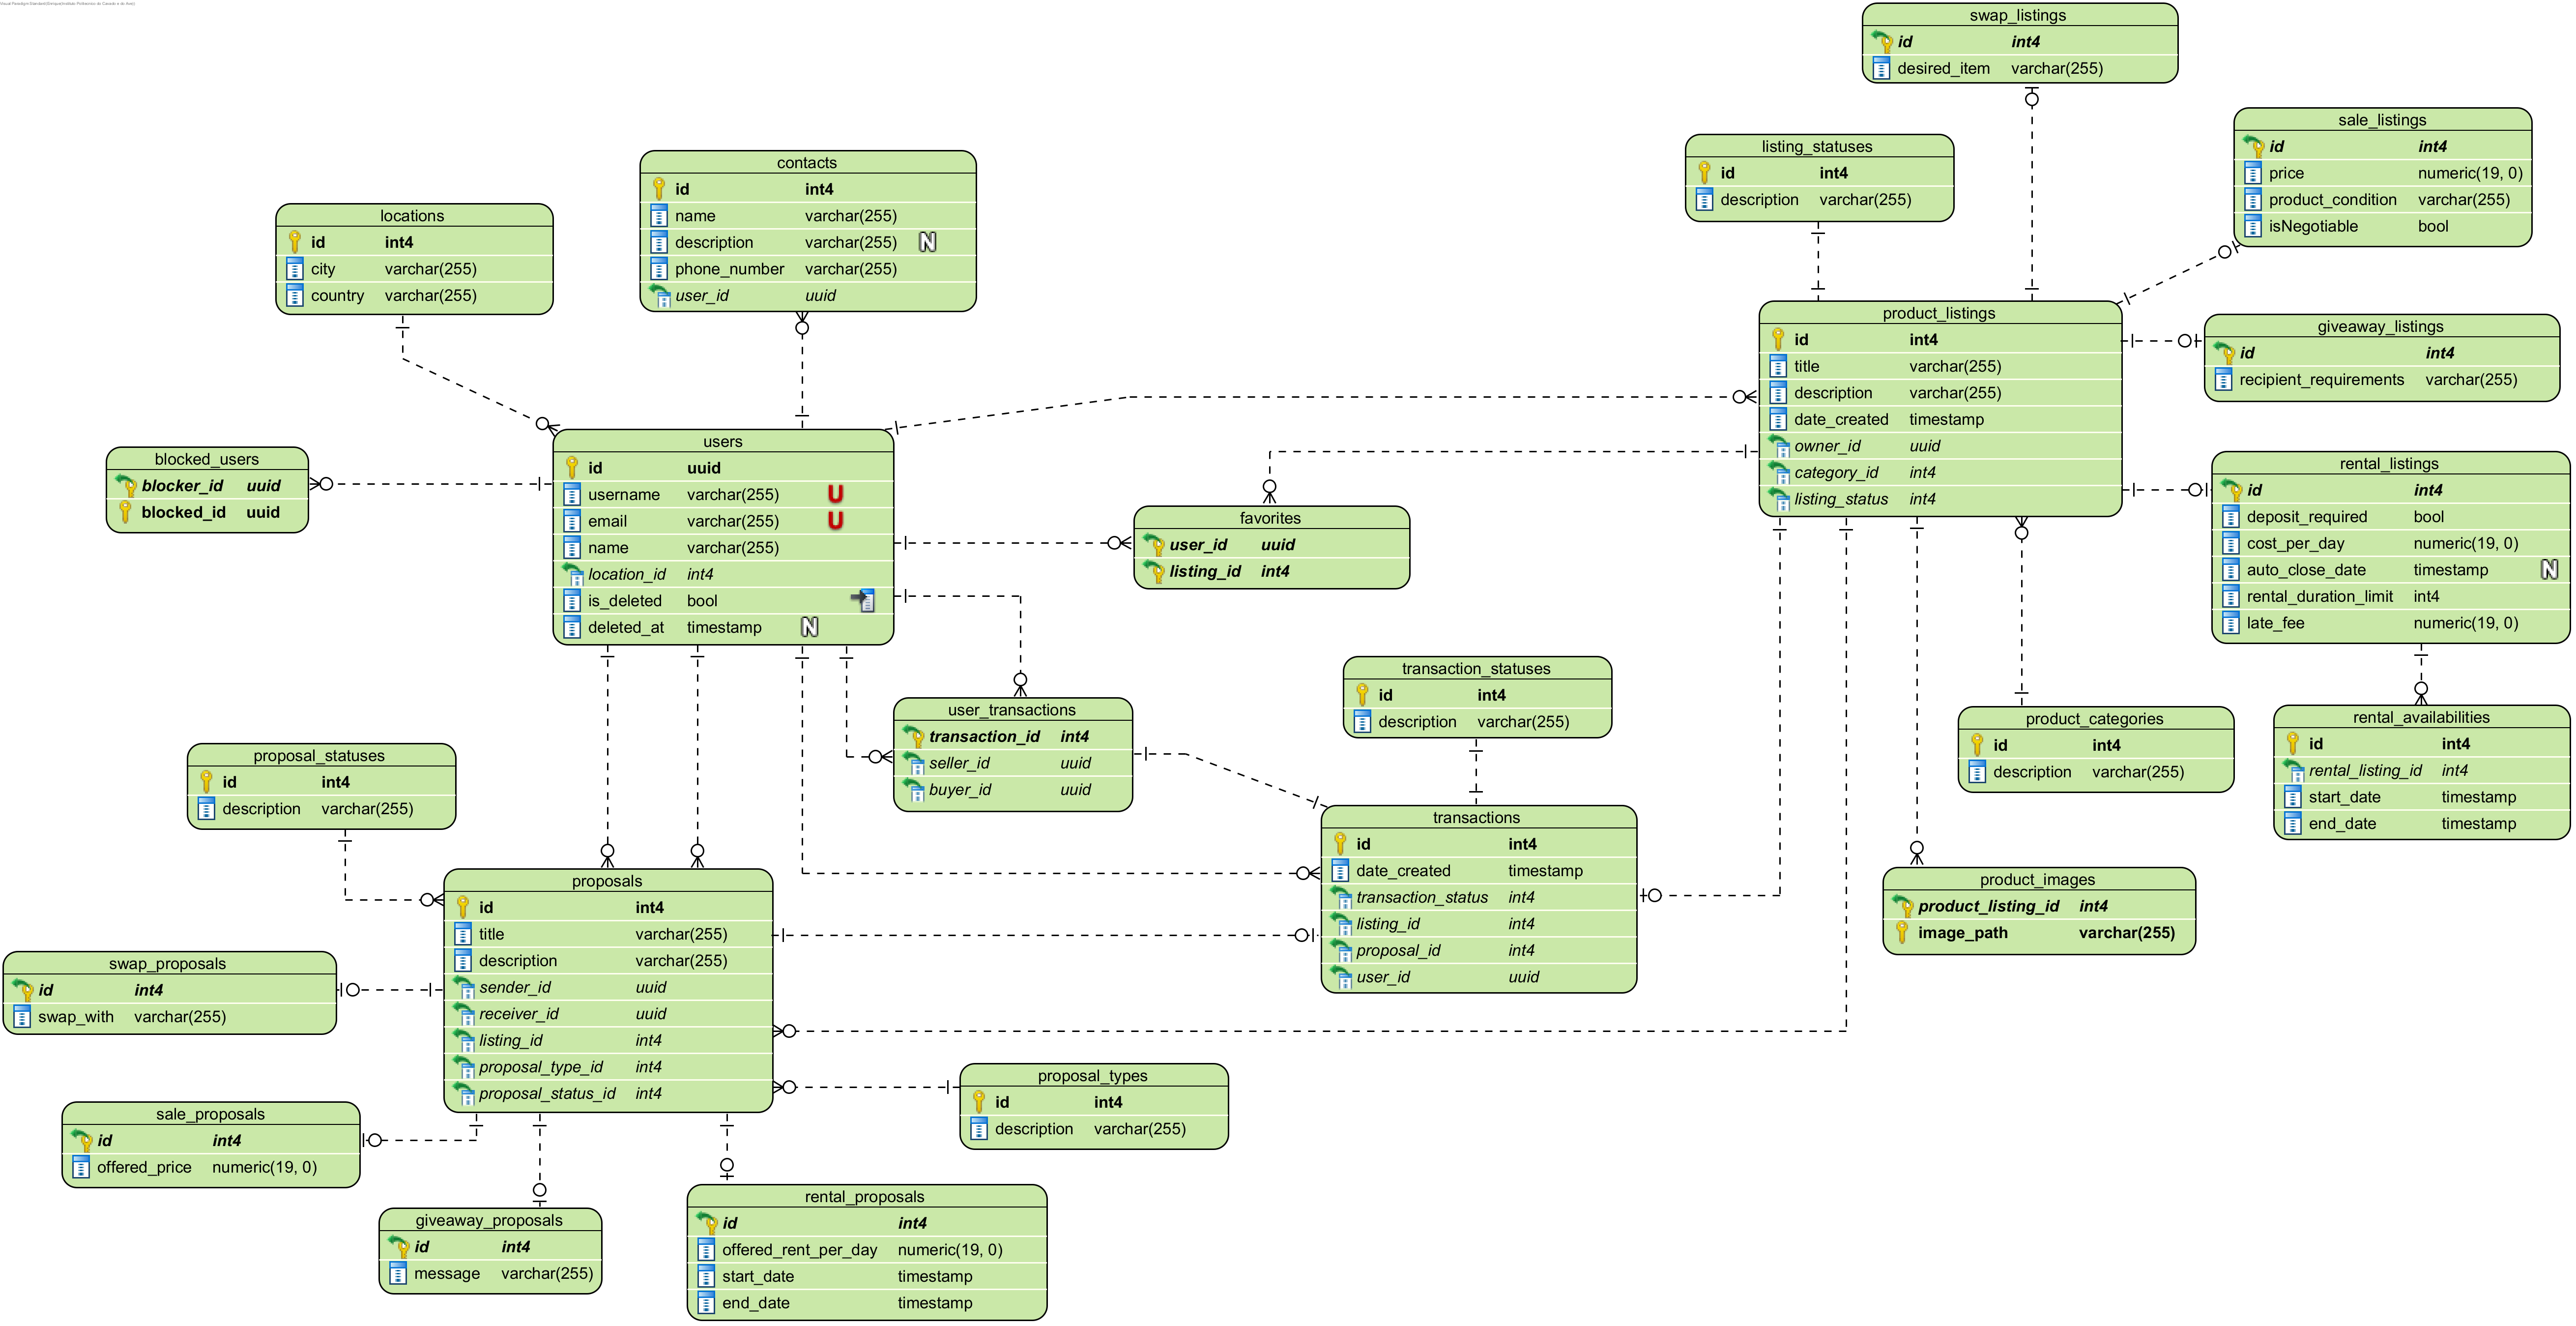
\includegraphics[width=\textwidth]{../images/entity-relationship-diagram.png}
	\caption{Diagrama ER}
	\label{fig:diagrama_er}
\end{figure}

%------------------------------------------------------------------------------------

\newpage
\section{Diagrama de Classes}

\subsection{Visão Geral}  

O diagrama de classes é uma representação visual da estrutura do sistema, demonstrando como suas classes se relacionam e interagem. É essencial para entender a organização do código, garantindo que o design da aplicação seja modular e bem estruturado.

Para isso, seguimos os princípios da \textit{Clean Architecture}, que ajudam a manter um código organizado, de fácil manutenção e escalável. Esta abordagem permite que cada classe tenha uma responsabilidade bem definida, separando claramente as camadas da aplicação e reduzir o acoplamento entre os componentes.

\subsection{Organização do Diagrama}  

O sistema está dividido em vários pacotes, cada um com uma função específica dentro da arquitetura. Esta estrutura facilita a manutenção, a testabilidade e a evolução do sistema. A seguir, apresentamos os principais pacotes e suas respectivas classes.

\subsection{Gestão de Utilizadores}

O pacote \textbf{User Management} trata da gestão dos utilizadores e das suas interações no sistema. Inclui as seguintes classes:

\begin{itemize}
	\item \textbf{User}: Representa um utilizador do sistema, contendo atributos como nome, email e localização. Além disso, um utilizador pode estar associado a vários \textbf{anúncios} (\textit{listings}) e \textbf{transações} (\textit{transactions}), permitindo rastrear os itens que publicou e as operações que realizou.
	\item \textbf{Contacts}: Gere a lista de contactos de um utilizador e fornece operações para adicionar e remover contactos.
	\item \textbf{BlockedUsers}: Permite bloquear e desbloquear utilizadores, garantindo maior controlo sobre interações indesejadas.
	\item \textbf{Favorites}: Mantém uma lista de itens favoritos do utilizador, facilitando o acesso rápido a listagens de interesse.
	\item \textbf{Location}: Representa a localização geográfica de um utilizador ou de um anúncio.
	\item \textbf{Company}: Atributo opcional associado a um utilizador, que indica a empresa à qual ele pertence.
\end{itemize}

Além destas classes, o pacote inclui várias \textbf{enumerações} para representar os resultados das operações, como por exemplo:

\begin{itemize}
	\item \texttt{BlockUserResult} – Indica o resultado de uma tentativa de bloquear um utilizador (sucesso, já bloqueado, não encontrado, erro).
	\item \texttt{AddContactResult} – Define os possíveis resultados ao adicionar um contacto (sucesso, já existe, contacto inválido, erro).
\end{itemize}

O uso de enumerações para representar estes resultados segue um princípio de \textbf{design limpo}, garantindo que as respostas das operações são bem definidas e evitam o uso de mensagens genéricas ou estados indefinidos. Com esta abordagem, o sistema mantém uma estrutura clara e consistente, facilitando a deteção e tratamento de erros através de códigos específicos.

%\begin{figure}[ht]
%	\centering
%	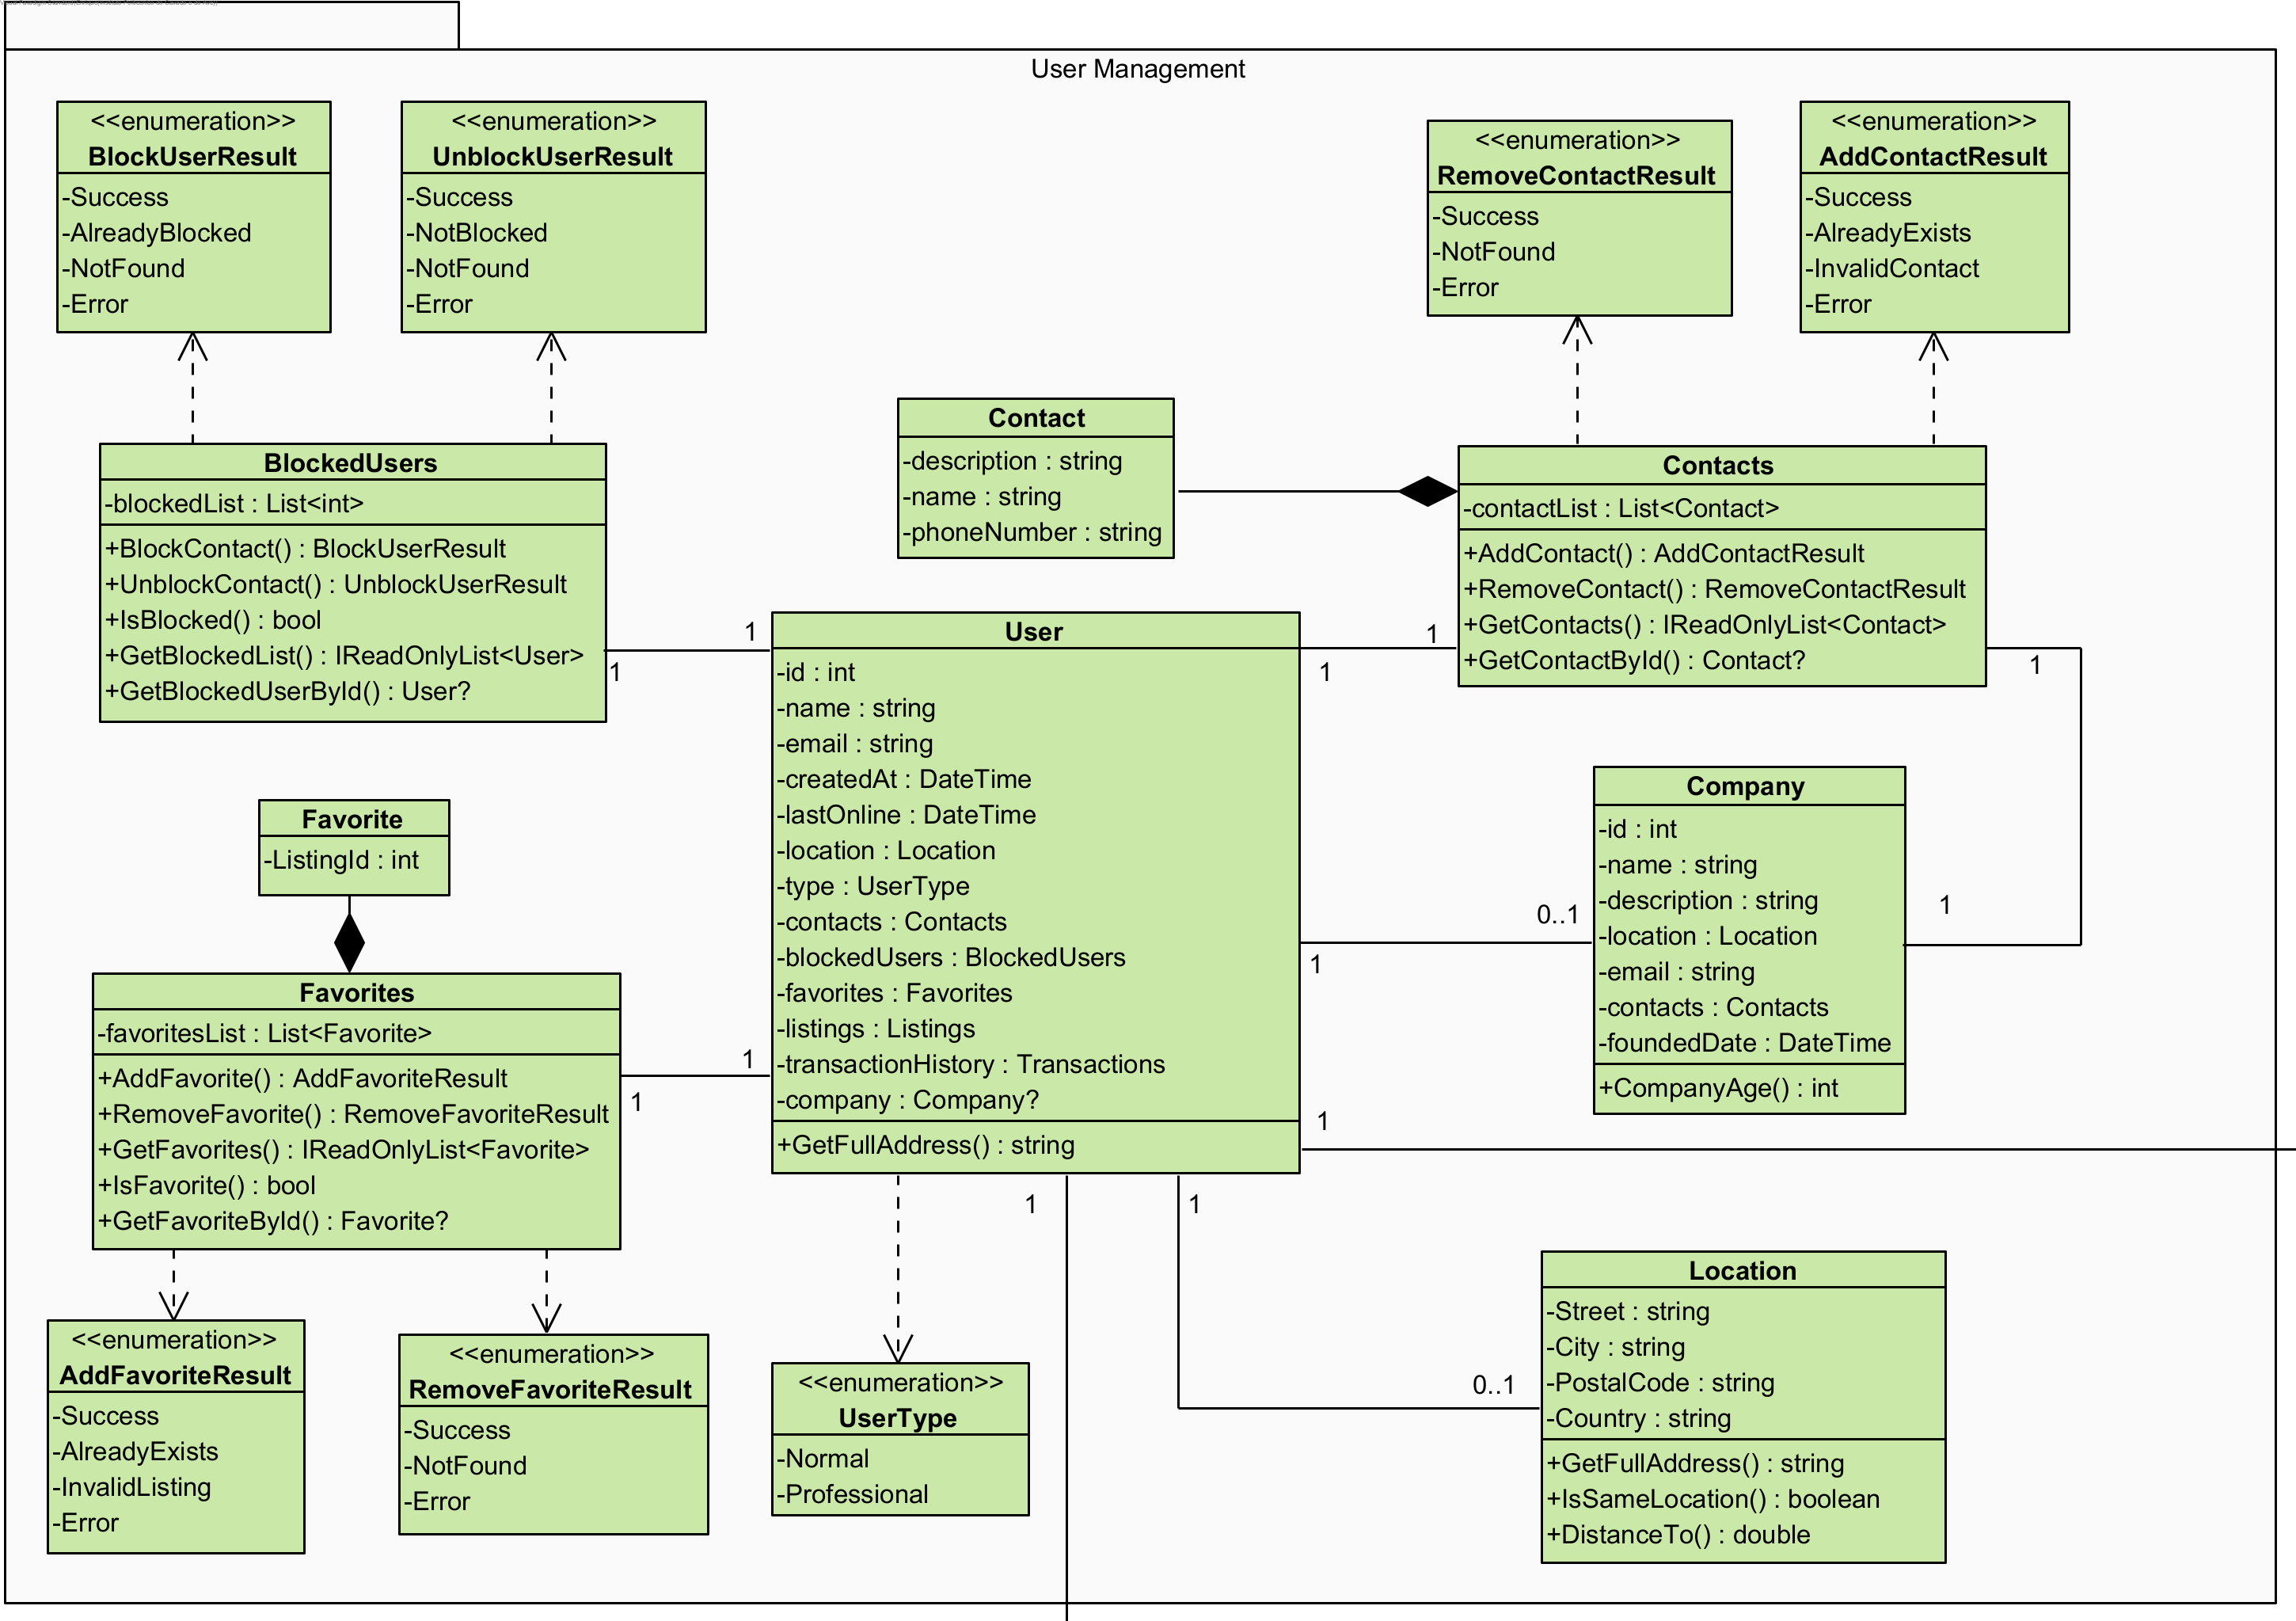
\includegraphics[width=\textwidth]{diagrama_classes_gestao_utilizadores.png}
%	\caption{Pacote de Gestão de Utilizadores}
%	\label{fig:diagrama_classes_gestao_utilizadores}
%\end{figure}


O pacote \textbf{Listings \& Items} é responsável pela gestão de anúncios e categorização de itens. Contém as seguintes classes:

\begin{itemize}
	\item \textbf{Listings}: Classe que contém uma lista de anúncios, oferecendo funcionalidades para adicionar, remover e pesquisar itens dentro dessa lista.
	\item \textbf{BaseListing}: Classe abstrata que serve de base para diferentes tipos de anúncios.
	\item \textbf{SwapListing}: Extende a classe \textit{BaseListing} e representa um item disponível para troca.
	\item \textbf{SaleListing}: Extende a classe \textit{BaseListing} e representa um item disponível para venda.
	\item \textbf{GiveawayListing}: Extende a classe \textit{BaseListing} e utilizado para itens oferecidos gratuitamente.
	\item \textbf{RentalListing}: Extende a classe \textit{BaseListing} e representa itens disponíveis para aluguer.
\end{itemize}

%\begin{figure}[ht]
%	\centering
%	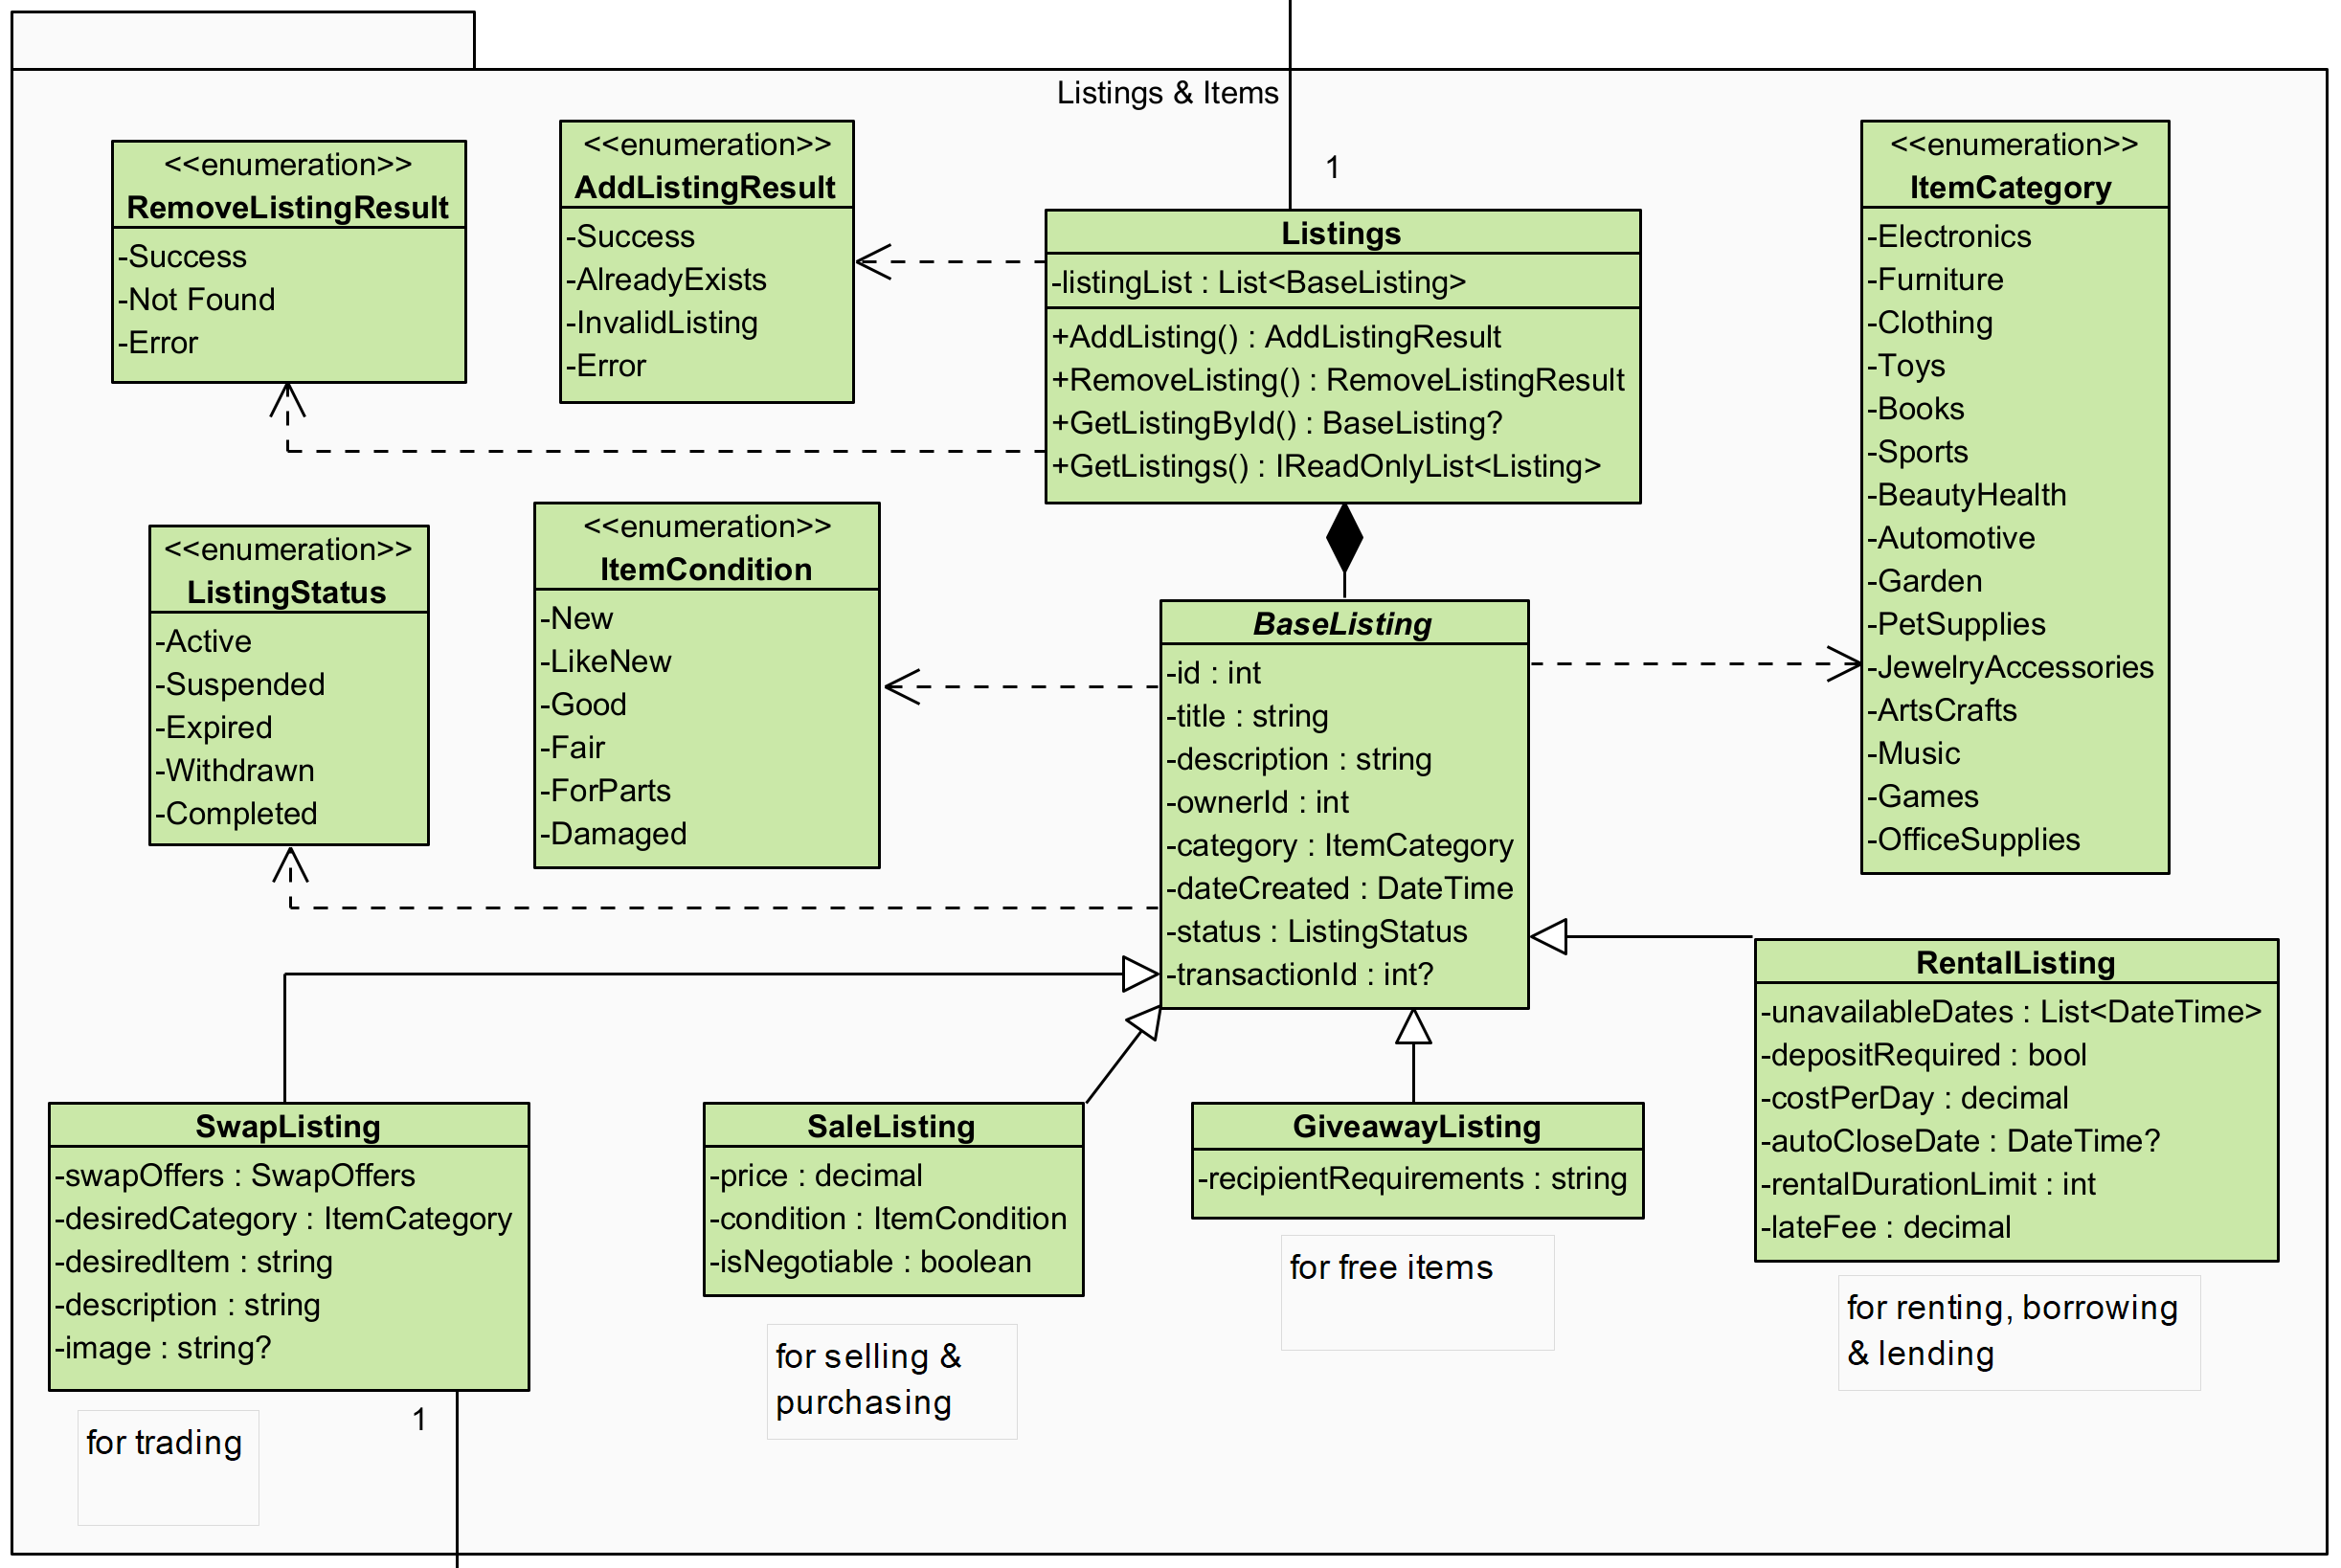
\includegraphics[width=0.9\textwidth]{diagrama_classes_anuncios_itens.png}
%	\caption{Pacote de Anúncios e Itens}
%	\label{fig:diagrama_classes_anuncios_itens}
%\end{figure}

\subsection{Transações}

O pacote \textbf{Transactions} gere as operações de compra, venda, troca e oferta de itens. Inclui:

\begin{itemize}
	\item \textbf{Transactions}: Classe que contém uma lista de todas as transações registadas no sistema.
	\item \textbf{BaseTransaction}: Classe abstrata que define a estrutura comum a todas as transações, com atributos como utilizador, item, data e status.
	\item \textbf{RentalTransaction}: Extende a classe \textit{BaseTransaction} e representa um aluguer de item entre utilizadores.
	\item \textbf{SaleTransaction}: Extende a classe \textit{BaseTransaction} e representa uma transação de venda.
	\item \textbf{SwapTransaction}: Extende a classe \textit{BaseTransaction} e permite a troca de itens entre utilizadores.
	\item \textbf{GiveawayTransaction}: Extende a classe \textit{BaseTransaction} e gere a oferta de um item sem custo.
\end{itemize}

%\begin{figure}[ht]
%	\centering
%	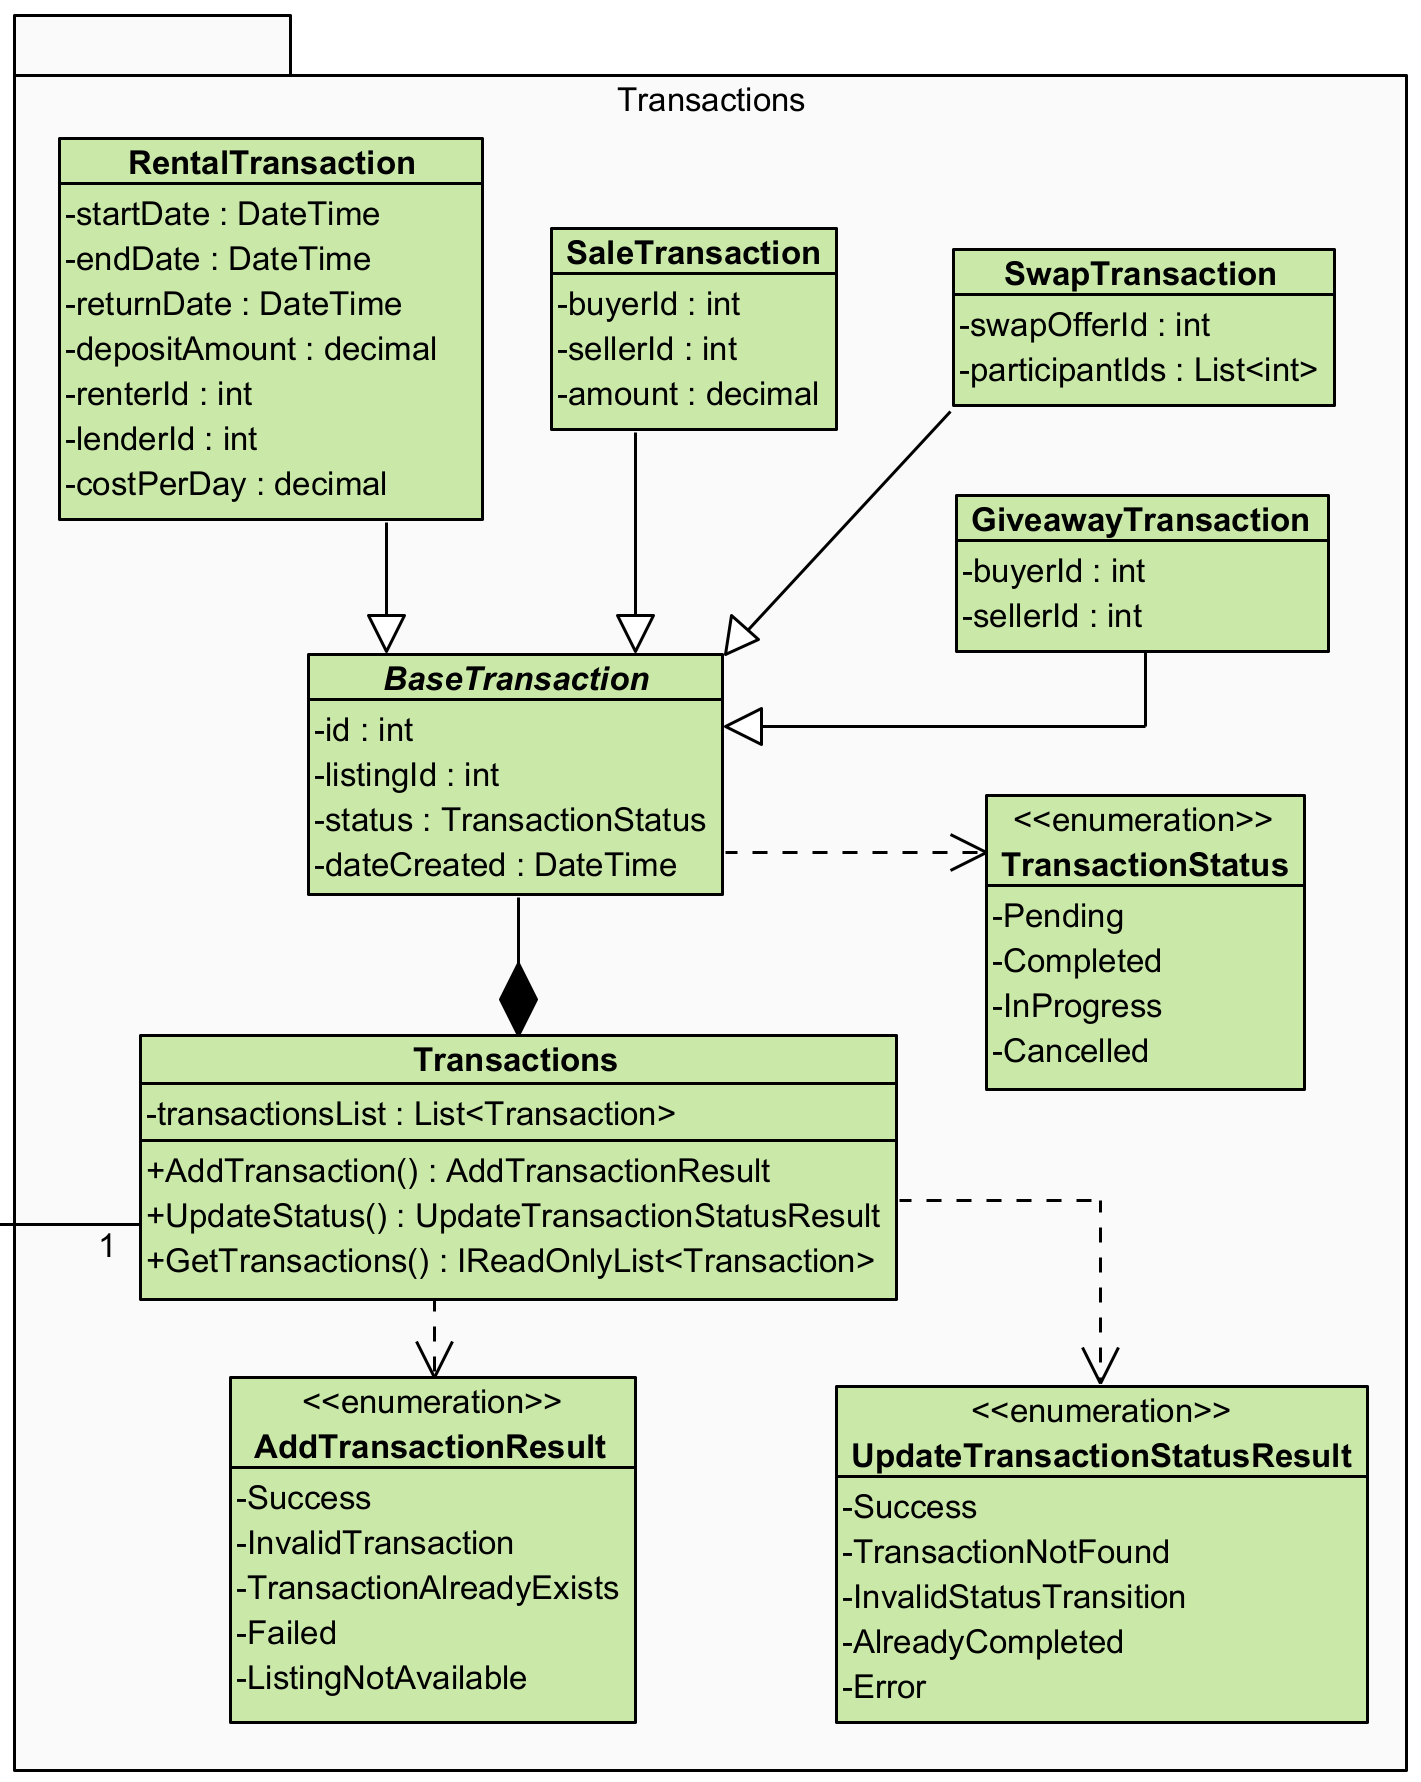
\includegraphics[width=0.53\textwidth]{diagrama_classes_transacoes.png}
%	\caption{Pacote de Transações}
%	\label{fig:diagrama_classes_transacoes}
%\end{figure}

\subsection{Trocas}

O pacote \textbf{Swaps} lida com a gestão de propostas de troca entre utilizadores. Inclui:

\begin{itemize} 
	\item \textbf{SwapOffers}: Contém uma lista de todas as ofertas de troca ativas no sistema. 
	\item \textbf{SwapOffer}: Representa uma proposta individual de troca entre utilizadores.
\end{itemize}

%\begin{figure}[ht]
%	\centering
%	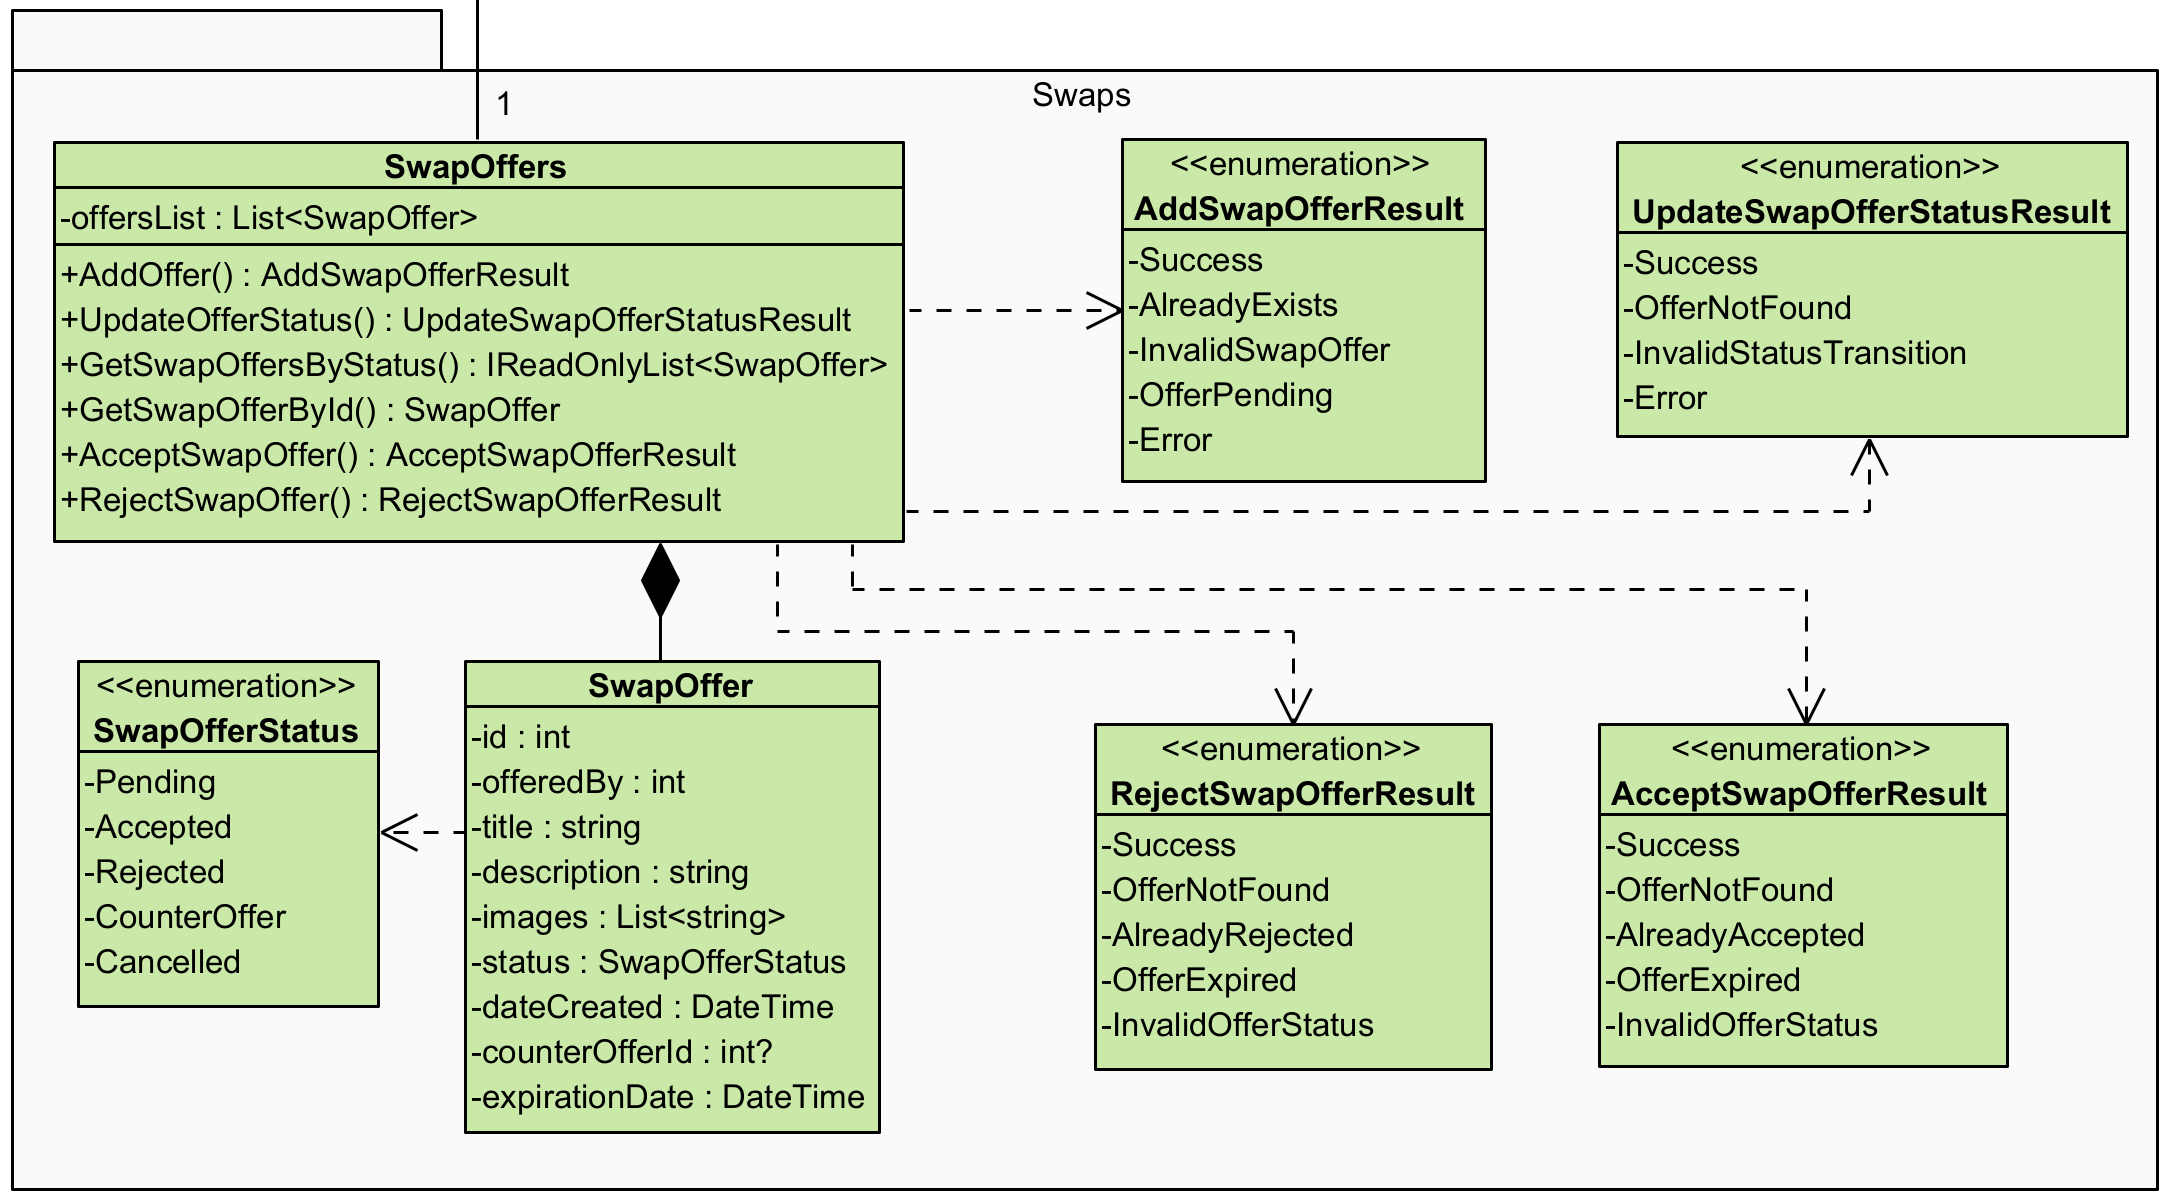
\includegraphics[width=\textwidth]{diagrama_classes_trocas.png}
%	\caption{Pacote de Trocas}
%	\label{fig:w}
%\end{figure}

\subsection{Relações entre os Pacotes}

Os pacotes interagem de forma a garantir a funcionalidade completa do sistema. A classe \texttt{User} está associada às \texttt{Transactions}, registando as operações realizadas pelos utilizadores, como compras, vendas, alugueres, trocas e ofertas. As \texttt{Listings} estão relacionadas com os utilizadores, representando os itens que estes publicam no sistema, seja para venda, troca, aluguer ou oferta. O pacote \texttt{Swaps} é responsável por gerir as propostas de troca entre utilizadores, estando diretamente ligado às \texttt{SwapOffer}. Cada pacote tem uma função bem definida, e as ligações entre eles garantem a coesão e eficiência do sistema.
%------------------------------------------------
\newpage
\section*{Diagrama de Sequência}

A plataforma pr

%------------------------------------------------
\newpage
\section*{Diagrama de Atividades}

A plataforma pr

%------------------------------------------------
\newpage
\section*{Design UI}

A plataforma pr

%------------------------------------------------
\newpage
\section*{Plano das Sprints para a Versão Alpha }

A plataforma pr

%------------------------------------------------
\newpage
\section*{Data da sprint Beta}

A plataforma pr

%------------------------------------------------
\newpage
\section*{Conclusion}

A plataforma proposta tem como objetivo criar um ambiente seguro e eficiente para a troca, venda e empréstimo de produtos dentro de uma comunidade. Ao permitir a marcação de encontros para a realização das transações, o projeto fomenta a interação entre os membros e incentiva práticas de consumo consciente. 
Com a definição clara dos requisitos e o suporte de diagramas UML e mockups, este relatório serve como um guia para o desenvolvimento da solução, garantindo que todos os aspectos essenciais sejam considerados.


%----------------------------------------------------------------------------------------
%	BIBLIOGRAPHY
%----------------------------------------------------------------------------------------

\bibliographystyle{unsrt}

\bibliography{sample}

%----------------------------------------------------------------------------------------

\end{document}